\subsection{Hierarchical model using cross-national, cross-sectoral data}

To measure corruption, FDI concentration, and treatment of firms across countries, I utilize the World Bank's Enterprise Survey (ES), which includes a wealth of firm-level data across 125 countries, spanning various topics from investment, labor, to business-government relation \citep{WorldBank2015}. The Enterprise Survey uses stratified random sampling (using three strata: firm size, business sector, and region) in order to ensure representativeness. The survey data comes from face-to-face interviews with upper management and is anonymized to ensure confidentiality at all times.\footnote{For more on the methodology of the Enterprise Survey, visit \url{http://www.enterprisesurveys.org/methodology}} This dataset has a wealth of firm-level data that helps us operationalize key concepts as detailed below.

Recall our hypothesis:

\begin{quote}
Hypothesis: High concentration of FDI in corrupt countries is associated with stunted domestic firms in those countries.
\end{quote}

\begin{quote}
Hypothesis: High concentration of FDI in corrupt sectors is associated with stunted domestic firms in those sectors.
\end{quote}

Operationalization:
\begin{itemize}
\item FDI in countries: available via UNCTAD data on FDI flows and stocks to countries. Concentration can be measured as the ratio of FDI to GDP.
\item FDI in sectors: available via the Enterprises Survey dataset. Concentration can be measured by constructing a Herfindahl-Hirschman Index based on the size of sale, labor, or capital of firms.
\item Corruption: can be measured in two ways. 1) Firms' perception about corruption as an obstacle. This measure is frequently used but the least accurate since firms' perception of corruption depends not only on the level of corruption but also the characteristics of firms. 2) Hard measure of prevalence and depth of bribes, e.g. ``Was an informal payment expected or request (when applying for a license)?'', ``How much do establishments like this one give in informal payments?''  

\item The development of the domestic private sector: can be measured by 1) experience of domestic firms with the business environment. However, this measure may simply capture the overall governance quality instead of showing that officials have neglected domestic firms to pursue rents with FDI firms. Therefore, a better measure is 2) the gap between the experience of domestic and foreign firms. This measure is also biased against our hypothesis, since foreign firms that self-select into investing (and thus show up in our survey sample) are more similar to domestic firms than foreign firms that decide not to invest.
\end{itemize}

\subsection{Cross-sectoral and sub-national variation in Vietnam}

Despite the wealth of firm-level, cross-national data in the ES dataset, it suffers from two fundamental issues.

First, its measure of corruption is still plagued by a host of measurement issues. Asking directly about firms' experience with corruption is unlikely to get an accurate answer due to sensitivity bias \citep{Coutts2011}. Researchers, including the ES team, often address this problem by framing the question about the experience with corruption of ``firms like yours.'' However, with this technique, firms may not read between the lines and actually answer about the experience of others \citep{Ahart2004}.

Second, since the development of the domestic sectors is a major factor why the government resorts to foreign firms for rents, its development matters in the sequencing of the game.

I can remedy these problems with a research design focusing on the case of Vietnam, taking advantage by a survey list experiment by \citet{Malesky2015}, which uses unmatched count technique to accurately measure the experience of firms with corruption while avoiding sensitivity bias.

Operationalization:
\begin{itemize}
\item FDI in province: Provincial statistics of FDI flow
\item FDI in sectors: PCI-FDI survey (can the survey sample be used to estimate the population's FDI?)
\item Corruption: list experiment \citep{Malesky2015}
\item Interest in promotion: 
\begin{itemize}
	\item years until retirement (retirement age is 60 for male, 55 for female)
	\item appearance in centrally controlled newspapers
\end{itemize}
\item The development of the domestic private sector:
\begin{itemize}
	\item PCI survey question: ``Do you think that the provincial officials prefer FDI?'' (Question H3)
	\item The gap in the experience of domestic and foreign firms regarding the pro-activeness of the government in helping business (Form H for domestic firms and Form J for foreign firms)
\end{itemize}
\end{itemize}

\begin{figure}[!ht]
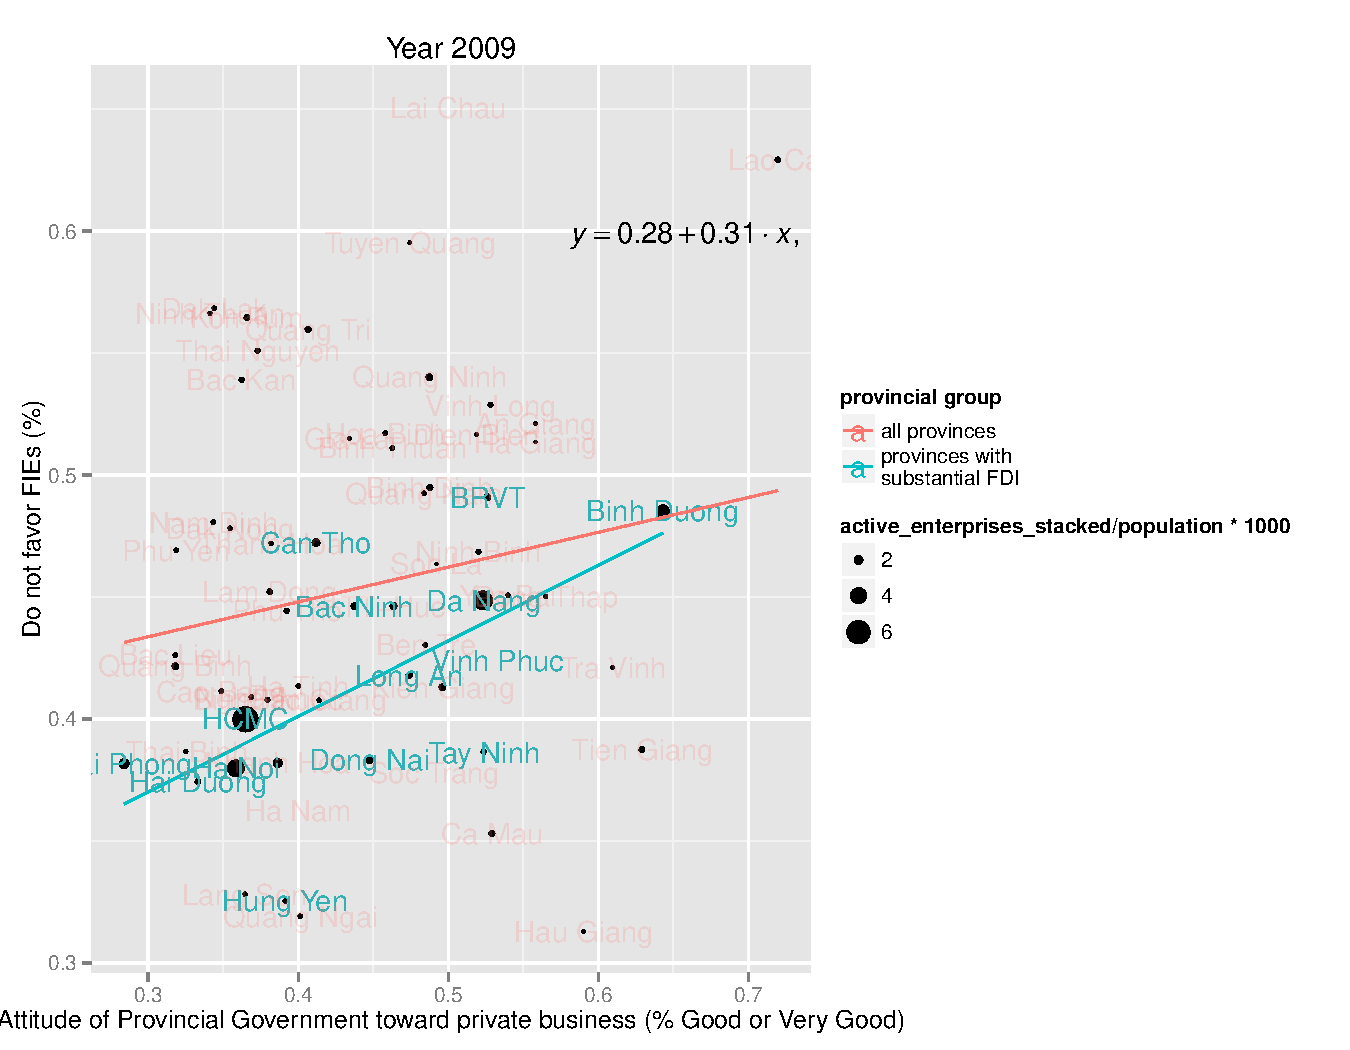
\includegraphics[width=\textwidth, height=\textheight,keepaspectratio]{../figure/FDI_bias}
\caption{The relationship between FDI bias and private sector development}
\label{fig:globalfdi}
\end{figure}


\subsection{Conjoint analysis}

While the crucial causal mechanism is the preference of provincial officials, observational data can only partially get at this because what the leaders want sometimes may not be fulfilled due to external factors (endowment, central policies). These factors can be controlled to some extent, yet the risk of mis-modeling is always present. Furthermore, what an official wants from a FDI firm is often hard to completely teased out. A big FDI firm is an attractive source of rent, but it also brings job and technology. Indeed, perhaps this high correlation is why it is so easy for officials to extract rent from FDI under the guise of promoting economic development.

To truly get at the preference of provincial leader, I plan to conduct a survey experiment using conjoint analysis to ask provincial officials about their preference between two hypothetical FDI firms \citep{Hainmueller2014}. The characteristics of these will be randomly varied across five dimensions: 1) industry, 2) size of labor force, 3) capital, 4) technology age, and 5) land, which proxies for corruption opportunities, since this is a key resource to firm that is controlled by provincial officials. If desired, it is possible to:
\begin{itemize}
\item adjust the design so that implausible hypotheticals will not appear (i.e. there should not be a high-tech company with very small capital).
\item randomize the ordering of the characteristics between respondents to test for the ordering effect (i.e. knowing a firm's industry first changes how the respondent thinks about the other characteristics)
\end{itemize}

I am mainly interested in the ``average marginal component effect'' (AMCE) of \textit{land}, which is the marginal effect of \textit{land} on the likelihood of a project being accepted, averaged over the distribution of all the other components. This allows us to back-out the what provincial officials truly want from FDI project.

\subsubsection{Experimental design}
Please read the following description carefully. Then, please indicate which project you prefer to grant investment license (cap giay phep dau tu).

\begin{center}
  \begin{tabular}{ c | c | c }
    \hline
     & Project 1 (Du an 1) & Project 2 (Du an 1) \\ \hline
    Industry &  &  \\ \hline
    Labor force &  &  \\ \hline
    Capital &  &  \\ \hline
    Land &  &  \\ \hline
    Technology age &  &  \\ \hline
    \hline
  \end{tabular}
\end{center}

If you have to choose, which project do you prefer to grant investment license? Project 1 / Project 2

\begin{itemize}
\item Industry: textile, electronics, automobile, consumer product
\item Labor force: 5, 50, 100, 200, 500 employees
\item Capital:
\item Land:
\item Technology age: 
\end{itemize}
